% ****** Start of file apssamp.tex ******
%
%   This file is part of the APS files in the REVTeX 4.1 distribution.
%   Version 4.1r of REVTeX, August 2010
%
%   Copyright (c) 2009, 2010 The American Physical Society.
%
%   See the REVTeX 4 README file for restrictions and more information.
%
% TeX'ing this file requires that you have AMS-LaTeX 2.0 installed
% as well as the rest of the prerequisites for REVTeX 4.1
%
% See the REVTeX 4 README file
% It also requires running BibTeX. The commands are as follows:
%
%  1)  latex apssamp.tex
%  2)  bibtex apssamp
%  3)  latex apssamp.tex
%  4)  latex apssamp.tex
%
\documentclass[%
 reprint,
%superscriptaddress,
%groupedaddress,
%unsortedaddress,
%runinaddress,
%frontmatterverbose,
%preprint,
%showpacs,preprintnumbers,
%nofootinbib,
%nobibnotes,
%bibnotes,
 amsmath,amssymb,
 aps,
 norsk,
 booktabs
%pra,
%prb,
%rmp,
%prstab,
%prstper,
%floatfix,
]{revtex4-1}

\usepackage[utf8]{inputenc}
\usepackage[norsk]{babel}
\usepackage{varioref}
\usepackage{graphicx}% Include figure files
\usepackage{enumitem}
\usepackage{dcolumn}% Align table columns on decimal point
\usepackage{bm}% bold math
\usepackage[margin=0.9in]{geometry}
\usepackage[mathlines]{lineno}% Enable numbering of text and display math
%\linenumbers\relax % Commence numbering lines

\usepackage[usenames,dvipsnames,svgnames,table]{xcolor}
\usepackage[colorlinks]{hyperref}
\usepackage{relsize}
%\usepackage{booktabs}
\usepackage{graphicx,verbatim,amsfonts,geometry}
\usepackage{amsmath}
\newcommand*\diff{\mathop{}\!\mathrm{d}}
\newcommand*\Diff[1]{\mathop{}\!\mathrm{d^#1}}
\usepackage{ulem}
\usepackage{amssymb}
\usepackage{soul}
\usepackage{dsfont}
\usepackage{commath}
\usepackage{wrapfig}
\usepackage[free-standing-units=true]{siunitx}
\DeclareSIUnit\year{yr}
\usepackage{gensymb}
\newcommand{\ROM}[1]{%
  \textup{\uppercase\expandafter{\romannumeral#1}}%
}
\usepackage{physics}
\usepackage{caption}
\usepackage{bm}
\usepackage{gensymb}

\makeatletter
\newcounter{elimination@steps}
\newcolumntype{R}[1]{>{\raggedleft\arraybackslash$}p{#1}<{$}}
\def\elimination@num@rights{}
\def\elimination@num@variables{}
\def\elimination@col@width{}
\newenvironment{elimination}[4][0]
{
    \setcounter{elimination@steps}{0}
    \def\elimination@num@rights{#1}
    \def\elimination@num@variables{#2}
    \def\elimination@col@width{#3}
    \renewcommand{\arraystretch}{#4}
    \start@align\@ne\st@rredtrue\m@ne
}
{
    \endalign
    \ignorespacesafterend
}
\newcommand{\eliminationstep}[2]
{
    \ifnum\value{elimination@steps}>0\sim\quad\fi
    \left[
        \ifnum\elimination@num@rights>0
            \begin{array}
            {@{}*{\elimination@num@variables}{R{\elimination@col@width}}
            |@{}*{\elimination@num@rights}{R{\elimination@col@width}}}
        \else
            \begin{array}
            {@{}*{\elimination@num@variables}{R{\elimination@col@width}}}
        \fi
            #1
        \end{array}
    \right]
    &
    \begin{array}{l}
        #2
    \end{array}
    \addtocounter{elimination@steps}{1}
}
\makeatother
% Document formatting
\setlength{\parindent}{0mm}
\setlength{\parskip}{1.5mm}

\begin{document}

\title{Måling av elastisitetsmodulen til messingstav med sirkulært tversnitt}
\author{\textsc{Ivar Svalheim Haugerud}}
\affiliation{ Universitetet i Oslo}
\date{\today}

\begin{abstract}
  Eksperimentelle målinger for å beregne elastisitetsmodulen til en sylindrisk messingstav ble gjennomført med to forskjellige utgangspunkter for å teste den fysiske modellen for elastisitet. Den ene metoden tok utgangspunkt i å måle statisk nedbøying av stavens midtpunkt som funksjon av belastning på midtpunktet til staven, mens staven hviler på to kniver. Den andre metoden baserte seg på å måle utbredelseshastigheten til frie longitudinelle svingninger i staven som oppstår ved slag i aksial retning. Det forventes at de to verdiene for elastisitetsmodulen er det samme for at det skal være en korrekt fysisk modell. De to verdiene for elastisiteten til messingstaven er henholdsvis
  $E=\SI{110\pm1}{\giga\pascal}$ og $\SI{109.3\pm0.3}{\giga\pascal}$. Differenasen mellom to de resultatene er $\SI{0.7\pm1.1}{\giga\pascal}$. Siden differansen mellom de to verdiene er mindre enn usikkerheten i differansen er det overenstemmelse innenfor måleusikkerhetene.
\end{abstract}

\pacs{Valid PACS appear here}% PACS, the Physics and Astronomy
                             % Classification Scheme.
%\keywords{Suggested keywords}%Use showkeys class option if keyword
                              %display desired
\maketitle

%\tableofcontents
\section{Introduksjon}
Eksperimentet i denne rapporten ble gjennomført i håp om å beregne elastistsmodulen til en sylindrisk messingstav på to måter, med forskjellig utgangspunkt, og ved dette teste kvaliteten på modellen for elastistet. En god modell burde kunne skrive flere fenomen med så få parametere som mulig. Vi skal derfor finne elastisitesparameteren, elastistsmodulen, ved å ta utgangspunkt i to forskjellige fenomener for å se om vi får samme verdi for elastistsmodulen.\\
Før vi går i nærmere detalj burde vi se mer på hva elastisitet er, og hva som menes med elastisitetsmodul. Elastisitet er egenskapen til et legme som gjør at legmet returnere til sin originale form etter å ha blitt utsatt  for ytre krefter \cite{gronn}. Dersom et legme kommer tilbake med nøyaktig samme form som før den ble utsatt for ytre krefter sier man at det er hundre prosent elastisk. Elastisiteten beskriver legmets evne til å oppta arbeid ved deformasjon, og bevare dette som potensiell energi som legmet bruker til å få sin opprinlige form når kraften opphører. Elastisitet blir også brukt om kollisjoner mellom legmer, hvor det beskriver hvor mye av bevegelsesenergien til legmene som er bevart mellom før og etter kollisjonen. Hvis det er et elastisk støt vil all kinetisk energi, hvis det er et uelastisk støt vil energi bli brukt til å deformere legmene i kollisjonen.\\

Når noe blir utsatt for spenning (\textit{stress}) vil tøyingen (\textit{strain}) generelt sett øke lineært med spenningen til det når et punkt som kalles \textit{elastisitetsgrensen}. Øker spenningen over elastisitetsgrensen vil legme ikke komme tilbake til sin opprinlige form når kraften opphører, deformasjonen slutter å være elastisk  \cite{gronn}. Øker spenningen enda mer kan man nå \textit{bruddgrensen} hvor legeme brytes i stykker. I dette eksperimentet kommer vi bare til å jobbe med spenninger mindre enn den som trengs for å nå elastisitetsgrensen, og vi forventer derfor et lineært forhold mellom tøyingen og spenningen i målingene våre.

Elastisitetsmodulen som vi kommer til å finne under eksperimentet, også kalt \textit{Young's modulus}, gir forholdet mellom spenningen som et legme blir utsatt for og den resulterende tøyingen til legmet. Og siden vi er under elastisitetsgrensen er forholdet lineært.

Det ene fenomenet vi skal se på for å finne elastisitetsmodulen er at objekter blir bøyd eller deformert når de blir utsatt for en kontinuerlig kraft. For å måle dette fester vi vekter midt mellom to punkter som staven hviler på og måler hvor mye staven blir bøyd . Med denne metoden finner vi sammenhengen mellom vekten vi bruker og avstanden staven blir nedbøyd.\\
Den andre metoden er å finne utbredelseshastigheten til longitudinelle bølger i staven. Ifølge teorien er utbredelseshastigheten avhengig av tettheten og elastisiteten til materialet. Vi kommer ikke til å måle utbredelseshastigheten direkte, men heller å begrense oss til en bølgelengde, og finne frekvensen til denne, som gjør at vi kan regne oss fram til hastigheten.\\
Dette er to fenomener som ifølge teorien bare beskrives av en parameter, som er et tegn på en god teori. Men teorien må selvfølgelig stemme med det vi observer for å være en god modell. Vi ønsker derfor å teste dette ved å måle elastistsmodulen med utgangspunkt i to forskjellige fenomener, som burde gi samme verdi for elastisitetsmodulen. Er de to verdiene vi finner innenfor usikkerhetene til hverandre har vi vist at det er en god modell. Hvis de to verdiene er ulike, utenfor usikkerhetene, kan det skyldes systematisk feil i eksperimentet eller feil i teorien. I dette tilfellet burde det bli gjennomført flere eksperimenter av samme type for å se nærmere på målingene.\\
Hensikten med en god modell for elastisitet er lett å se nytten av. Elastisitet spiller en stor rolle for byggkonstruksjoner, for forståelsen av vibrasjoner, for forplantning av lyd og for studiet av kreftene mellom atomer eller molekyler i krystallgittere \cite{gronn}. For eksmepel ønsker byggningsingeniører å forutsi hvor mye en struktur klarer å bære før det ikke er trygt lenger, og denne vitenskapen baserer seg på en god forståelse av elastisiteten til materialene man bruker. Om man måtte teste eksperimentelt for hvert hus, blokk, bil eller båt som blir bygd hvor mye det tåler før det ikke lenger er trygt, ville det vært ekstremt tidkrevende og uøkonomisk oppførsel. Med en god fysiskmodell vil man slippe dette, og vi kan leve livene våre uten å bekymre oss for at alt, fysisk, rundt oss kommer til å rase.
\section{Teori}
\subsection{Måling av nedbøying}
Nedbøyingen $h(m)$ til en bjelke, som støtter seg på to punkter med avstand $l$, som bærer en last på $mg$ i midten av bjelken gitt ved
\begin{equation}
  h(m) = \frac{mgl^3}{48EI}.\label{young}
\end{equation}
I dette uttrykket er $E$ elastisitetsmodulen og $I$ er arealtreghetsmomentet til bjelken, ikke massetreghetsmomentet som brukes i dynamikk. Arealtreghetsmomentet, også kalt andre arealmoment, er integralet over tversnittet til bjelken
\begin{equation*}
  I = \int\int x^2 \diff x \diff y,
\end{equation*}hvor bjelken strekker seg ut i $z$-retning, og lasten virker i $x$-retning. For eksperimentet vi skal gjøre kommer bjelken til å være en sylinder. Vi kan derfor beregne arealtreghetsmomentet til en sylinder med radius $R$. Vi beregner integralet i sylinderkoordinater, og multipliserer derfor med jacobideterminanten, og bruker at $x = r\sin{\theta}$. Vi får
\begin{equation*}
  I = \int_0^{2\pi} \int_0^R r^2\sin^2{\theta}r \diff r \diff \theta = \frac{\pi r^4}{4} = \frac{\pi d^4}{64},
\end{equation*}
der $d$ er diameteren. Setter vi dette inn i \eqref{young} får vi
\begin{equation*}
  h = \frac{4mgl^3}{3\pi Ed^4}.
\end{equation*}
Siden vi er interesert i å måle elastisitetsmodulen til bjelken kan vi løse for likningen for $E$ for å få
\begin{equation}
  E = \frac{4mgl^3}{3\pi hd^4}. \label{young2}
\end{equation}
Under eksperimentet kommer vi til å måle nedbøyingen $h$ som en funksjon av lasten $m$, der vi forventer har en lineært forhold
\begin{equation*}
  h(m) = \alpha m + \beta.
\end{equation*}
Konstantleddet $\beta$ vil være tilnærmet lik null siden staven ikke vil være bøyd med null last, og vi kan derfor erstatte $h/m$ med stigningstallet $\alpha$ som vi vil beregne under målingene. Setter vi dette inn i \eqref{young2} får vi et uttrykk for elastisitetsmodulen til en sylinderformet stav er
\begin{equation}
  E = \frac{4gL^3}{3\pi \alpha d^4}. \label{young3}
\end{equation}
Under eksperimentet kan vi måle alle de ukjente variablene i uttrykket slik at vi får en verdi for elastisitetsmodulen til messing.\\
%For å finne tyngdeakselerasjonen i Oslo bruker vi \textit{gravitational latitude formula} som tar hensyn til breddegrad og høyde over vannet. Man beregner da tyngdeakselrasjonen med
%\begingroup\makeatletter\def\f@size{8.5}\check@mathfonts
%\begin{align}
%\begin{split}
%  g =  &\SI{9.780327}{\meter s^{-2}}\left(1 + 0.0053024 \sin{2\Phi} – 0.0000058 \sin^2{2\Phi}\right)\\ &-\SI{3.086e-6}{s^{-2}} \cdot h,
%\end{split}
%\end{align}
%\endgroup
%der $h$ er høyden over havet, og $\Phi$ er breddegraden.
\subsection{Måling av utbredelseshastigheten til bølger}
Vi ønsker å bruke en annen metode for å finne elastisitetsmodulen. Denne metoden for bestemmelse av E baserer seg på å finne utbredelseshastigheten $v$ for longitudinalbølger i en stav. Vi kan bruke dette som utgangspunkt siden utbredelseshastigheten er avhengig av elastistsmodulen ved
\begin{equation}
  v = \sqrt{\frac{E}{\rho}},\label{vel}
\end{equation}
hvor $\rho$ er mediets tetthet. Siden massetetthet er masse per volum kan vi finne $\rho$ ved å måle massen og volumet til staven, og beregne tettheten fra
\begin{equation*}
  \rho = \frac{4M}{\pi L d^2},
\end{equation*}
hvor $L$ er lengden på hele staven. Vi kan sette dette inn for $\rho$ i \eqref{vel} og løse for $E$, som gir oss
\begin{equation}
  E = \frac{4Mv^2}{\pi L d^2}.\label{elast}
\end{equation}
For å kunne beregne elastisitetsmodulen mangler vi bare utbredelseshastigheten i staven. Denne kan vi bestemme ved å måle verdien til frekvens $f$ og bølgelengden $\lambda$, som gir oss utbredelseshastigheten ved sammenhengen
\begin{equation}
  v = \lambda f.\label{vlf}
\end{equation}
%Både bølgelengde og frekvens kan bestemmes ved måling på en stående bølge i staven.
Det kan vises at ved frie longitudinelle svingninger i en homogen stav med lengde $L$ opphengt i midtpunktet og med frie ender, får vi svingninger slik at
\begin{equation*}
  L = \frac{n\lambda}{2},
\end{equation*}
der $n$ er et oddetall $n = 1, 3, 5, \ldots$ Dette kan løses for bølgelengden $\lambda$, som gir oss en sammenheng mellom bølelengden og lengden av staven
\begin{equation*}
  \lambda = \frac{2L}{n},
\end{equation*}
Ved å slå staven i aksial retning dannes det flere egensvingninger i staven. Av disse svingningene er det den med lengst bølgelengde, $\lambda = 2L$, som blir mest dominerende som tiden går. Ved noen lenger til staven vil disse frekvensene gi hørbar lyd. Under eksperimentet kommer dette til å være tilfellet, og vi kan høre lyden fra frekvensen. Siden svingningen med lengst bølgelengde er den mest dominerende, og derfor hører tydeligst og lengst, vil det være den svingningen vi fokuserer på videre ved å velge $n=1$ og får
\begin{equation}
  \lambda = 2L.
\end{equation}
Setter vi dette inn for bølgelengden i \eqref{vlf} og får vi
\begin{equation*}
  v = 2Lf,
\end{equation*}
som vi kan sette inn for utbredelseshastigheten i \eqref{elast} får vi
\begin{equation}
  E = \frac{16MLf^2}{\pi d^2}. \label{young5}
\end{equation}
Ved å kunne måle de geometriske størrelsene og massen til staven, og frekvensen når vi slår på den, klarer vi å beregne elastisitetsmodulen med utgangspunkt i et annet fenomen. Hvis man istedenfor ønsker å finne frekvensen kan man gjøre dette ved å vite elastisitetsmodulen, massen og de geometriske størelsene til staven ved
\begin{equation}
  f = \sqrt{\frac{\pi E d^2}{16ML}}. \label{young6}
\end{equation}
\subsection{Usikkerheter}
På grunn av usikkerhet i målingene forventer vi ikke nøyaktig like svar for elastisitetsmodulen med de to metodene. Det er derfor viktig å vite usikkerhetene i de to metodene. Ved å bruke uttrykket for nedbøying av staven \eqref{young3} får vi at usikkerheten i elastisitetsmodulen er
\begingroup\makeatletter\def\f@size{7.5}\check@mathfonts
\begin{equation}
  \Delta_{E_1} = E_1 \sqrt{\left(3\frac{\Delta_L}{L}\right)^2+\left(\frac{\Delta_g}{g}\right)^2+\left(\frac{\Delta_A}{A}\right)^2+\left(4\frac{\Delta_d}{d}\right)^2},\label{uncertenty1}
\end{equation}
\endgroup
hvor konstantleddet forran $L$ og $d$ kommer fra eksponten de har i uttrykket.
Usikkerheten ved å bruke utrrykket for elastistsmodulen ved måling av frekvens \eqref{young5} er
\begingroup\makeatletter\def\f@size{7.5}\check@mathfonts
\begin{equation}
  \Delta_{E_2} = E_2 \sqrt{\left(\frac{\Delta_M}{M}\right)^2+\left(\frac{\Delta_L}{L}\right)^2+\left(2\frac{\Delta_f}{f}\right)^2+\left(2\frac{\Delta_d}{d}\right)^2}. \label{uncertenty2}
\end{equation}
\endgroup
Som sagt forventer vi ikke at de to metodene skal gi at differanse til elastisitetsmodulen $$D=\abs{E_1-E_2}$$ skal være null, hvor $E_1$ og $E_2$ er de to forskjellige verdiene vi får i vår utregning av elastistsmodulen ved våre to forskjellige metoder. Men vi ønsker at differeansen $D$ skal være mindre enn usikkerheten i differansen $\Delta_D$. Når vi har gjort målingene må vi derfor sjekke om de tilfredstiller
\begin{equation}
  D < \Delta_D, \label{usikk1}
\end{equation}
der
\begin{equation}
  \Delta_D = \sqrt{\Delta_{E_1}^2 + \Delta_{E_2}^2}. \label{usikk2}
\end{equation}
Hvis målingene våre tilfrestiller denne ulikheten kommer årsaken til differansen $D$ fra usikkerheterer i målemetoden og tilfeldige feil. Hvis dette er tilfellet sier vi at det er
\textit{overenstemmelse innenfor måleusikkerhetene}.
Derimot hvis
\begin{equation}
  D > 2\Delta_D
\end{equation}
er det lite sansynlig at det bare er tilfeldige feil og usikkerheter i målinger som er årsaken til feilen, da er det mest sansynlig systematiske feil som har forårsaket forskjellen mellom de to svarene vi fikk for elastistsmodulen med de to metodene.
\section{Metode}
\subsection{Nedbøying av messingstav}
I eksperimentet vårt bruker vi en messingstav med sirkulært tversnitt som er mye lenger enn diameteren sin. Vi ønsker først å måle elastisitetsmodulen ved å måle nedbøying av messingstaven når vi fester vekter på midten av staven. Oppsettet brukt i dette eksperimentet er vist i figur \vref{eksperiment}. I eksperimentet bruker vi en messingstav $E$ som hviler på to kniver $B$ og $C$. Midt på messingstaven er det festet en holder $F$ hvor vi setter loddene på. Ved måleuret $G$ kan vi måle bøyingen avmessingstaven. Hele eksperimentet foregår på en plate $A$.\\
Før vi begynner eksperimentet er det viktig at at holderen $F$ er festet midt mellom de to knivene. Vi måler derfor avstanden mellom $B$ og $C$ og flyttet på staven slik at midten av staven var halvparten av denne avstanden fra $B$. For å sjekke at alt var gjort korrekt gjorde vi målingene på nytt, men nå målte vi avstanden fra $B$ til $F$ og fra $F$ til $B$ som gir oss mindre usikkerhet. Fra dette kunne vi finjustere posisjonen til staven til vi var sikkre på den var sentrert riktig. Itilegg er det viktig at punktet hvor nålen fra måleuret treffer normalt på flaten til sylinderen. For å være sikker på at den er normalt på kan vi bruke et vater og justere til vi er fornøyde.\\
Målet vårt er å bruke \eqref{young3} til å beregne elastisutetsmodulen, og for å gjøre dette trenger vi å vite både lengden av staven og diameteren. Vi bruker derfor et skyvelær til måle diameteren til staven. Siden staven er mye lengere i lengden enn i bredden måtte vi bruke en meterstokk. Siden disse verdiene er i tredje og fjerde potens er det viktig å gjøre presise målinger, siden usikkerhetene her vil ha store utslag i usikkerheten i det endelige resultatet. Vi trenger også å finne en nøyaktig verdi tyngdeakselerasjonen $g$, og usikkerheten i denne verdien. Denne verdien kan variere avhengig av hvor på kloden man er, og vi må derfor finne en verdi for Oslo, Norge. \\
Nå som eksperimentet er klart for måling, men før vi kan begynne må vi kalibrere loddene med presisjonsvektene. For å kalibrere loddene bruker vi en balansevekt, og setter den i likevekt med presisjonsvektene, for så å bytte presisjonsvektene ut med loddene og måle avviket mellom dem.
Når dette er gjort er alt klart for å måle nedbøyingen av staven.\\
Vi leser av nedbøyingen av staven som en funksjon av massen til loddene vi legger på festepunktet. Mellom hver måling tar vi av loddene og sjekker at utslaget til måleuret er tilbake til $0$-punktet. Massene vi har valgt å bruke går fra $0$ til $3.5$kg med en lineær økning på $0.5$kg. På disse målingene forventer vi et lineært forhold mellom vekten på loddene og nedbøyingen. For å bruke \eqref{young3} trenger vi stigningstallet til målepunktene, som vi kan beregne fra minste kvadraters metode på målingene. \\
\begin{figure*}
  \centering
  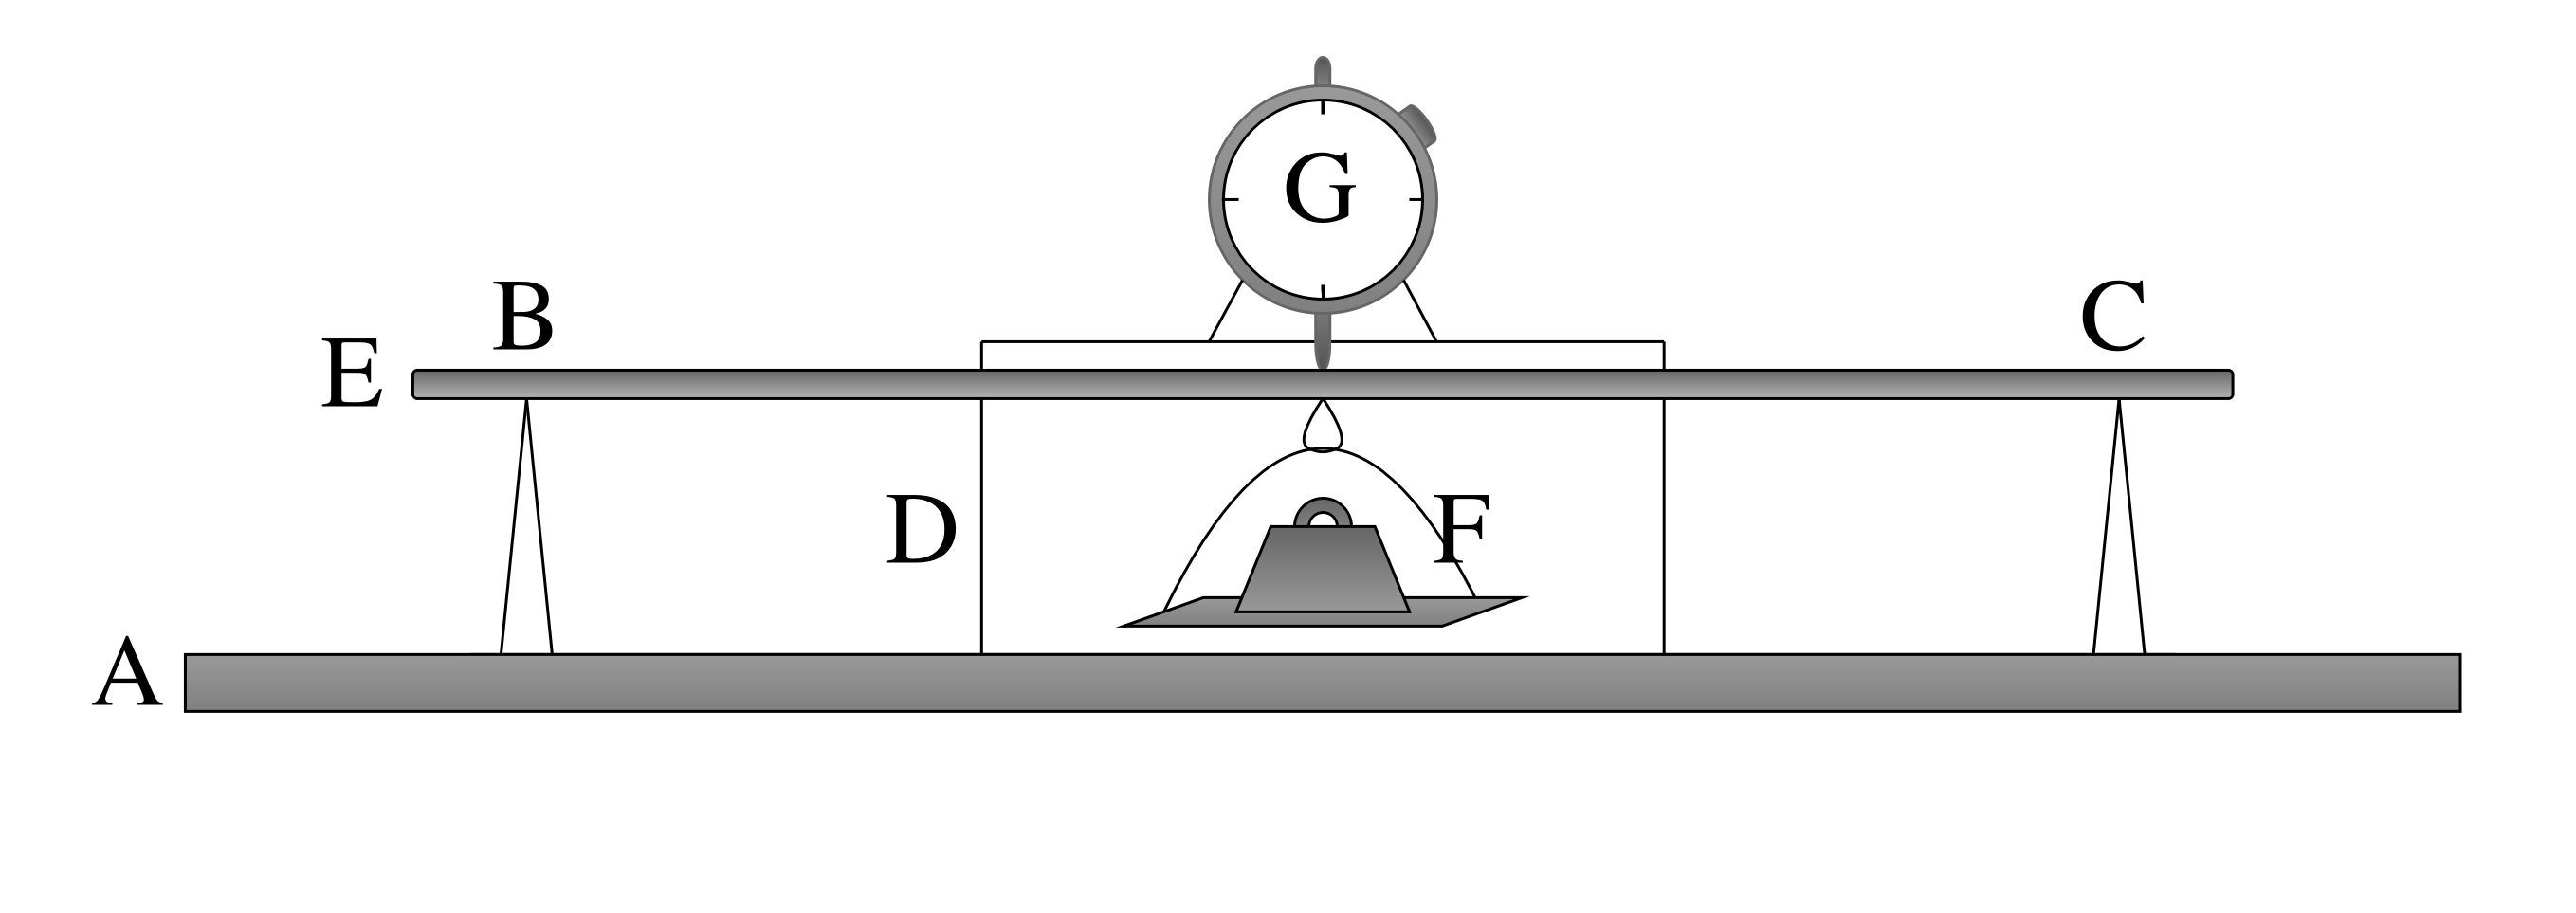
\includegraphics[scale=0.17]{oppsett.png}
  \caption{Eksperimentelt oppsett for målinger. Illustrasjon av staven som hviler på to knvier, med et måleur som måler nedbøyingen av stavens midtpunkt. På stavens midtpunkt fester vi loddene for å måle nedbøying som funksjon av belastningen.}
  \label{eksperiment}
\end{figure*}
\subsection{Måling av utbredelseshastigheten til bølger}
For å beregne elastisitetsmodulen ved å måle frekvensen til trykkbølger i staven bruker vi likning \eqref{young5}. Vi trenger derfor å vite diameteren og lengen til staven, men disse verdiene har vi allerede målt. Vi kan derfor måle massen. For å veie bruker vi balansevekten som vi har kalibrert tidligere. For å holde staven stabil på vekten måler vi den med et balanse ledd som vi trekker fra den totale massen for å finne massen til staven. Vi lar staven henge horisontalt og gir den et slag aksialt på med en plastikk hammer. Dette slaget danner trykkbølger i staven hvor den mest dominerende vil være den med kortest bølgelengde. For å måle frekvensen er det to forskjellige fremgangsmåter, fouriertransformasjon eller svevning.\\
For å bruke fouriertransformasjon bruker vi en mikrofon som vi setter nære staven. Fra et matlabprogram som leser signalene fra mikrofonen og tar en fouriertransformasjon av signalene, kan vi velge en samplingsfrekvens og en samplingstid for målingen. Etter slaget på staven venter vi litt før vi starter målingen med mikrofonen siden de andre frekvensene enn den med lengst bølgelengde dør ut først. Ved å finne en verdi for frekvensen med denne metoden har vi alle verdiene vi trenger for å beregne elastisitetsmodulen ved likning \eqref{young5}.\\
For å bruke sveve-metoden antar vi en verdi for frekvensen til trykkbølgene og bruker denne frekvensen i en høytaler som sender en tone med samme frekvens. Hvis frekvensen vi hører fra høytaleren er nesten lik frekvensen vi hører fra å slå på staven vil det oppstå en effekt som kalles svevning. Denne svevningen er lett å høre, og jo nærmere frekvensene er hverandre vil tidsavstanden mellom to perioder i svevningen øke. For å gjøre det lettere å høre svevningen burde styrken fra høytaleren være rundt samme styrke som den fra staven. Vi kan med denne metoden endre på frekvensen til signalet fra høytaleren mens vi hører signalet fra staven. Hvis vi starter med en frekvens og endrer den slik at perioden på svevningen øker kan vi endre frekvens i samme retning til svevningen er helt borte. Når svevningen er helt borte har vi funnet frekvens til signalet. Med denne metoden er det vanskelig å beregne en usikkerhet i frekvensen. Å velge en frekvens til høytaleren kan gjøres ved å først bruke fouriertransformasjons-metoden ovenfor for å finne en frekvens, og så velge samme frekvens på høytaleren, eller bruke likning \eqref{young6} hvis man har elastisitetsmodulen.
\section{Resultater}
Målingene av messingstaven som vi brukte i eksperimentet, usikkerheten i målingene og måleinstrument, er vist i tabell \vref{stav}. Dette er all informasjonen vi trenger å vite om messingstaven, som vi trenger for begge metodene å måle elastistsmodulen på.
\begin{table}[h!]
\centering
\caption{Målinger gjort av de geometriske størrelsene til messingstaven. Usikkerhetene er hentet fra databladet til måleinstrumentene.}
\label{stav}
\begin{tabular}{cccc}
    Egenskap & Målt verdi      &    Usikkerhet & Måleinstrument \\
    \hline
    Lengde $L$ [m] & $1.490$    & $\pm 0.004$  & meterstokk  \\
    Avstand kniver $l$ [m] & $1.365$ & $\pm0.004$ & meterstokk \\
    Diameter $D$ [cm] & $1.596$    & $\pm0.003$ & skyvelær    \\
    Masse $M$    [kg]  & $2.5173$   & $\pm0.0006$   & balansevekt \\  \hline
\end{tabular}
\end{table}
\subsection{Måling av nedbøying}
For å bruke likning \eqref{young3} trenger vi å vite de geometriske størrelsene til staven vist i tabell \vref{stav}, itillegg til tyngdeakselerasjonen $g$. Verdien for Tyngdeakselerasjon $g$ beregner vi fra \textit{International gravitational formula (IGF)} som tar hensyn til breddegrad itillegg til høyde over havet \cite{gravity}. Ved å bruke at høyden over havet i fysikkbygget er $\SI{90}{\meter}$ og at Oslo har en breddegrad på $59.91\degree$, som gir oss at tyngdeakselrasjonen er $g=\SI{9.819\pm0.005}{\meter\per\second^2}$. Usikkerheten kommer fra modellen brukt til å beregne tyngdeakselrasjonen \cite{gravity}.
Nå som vi har tyngdeakselerasjonen er det eneste vi mangler for å finne elastistsmodulen stigningstallet $\alpha$ fra målingene av nedbøyingen. Målingene vi brukte for å beregne stigningstallet er vist i figur \vref{data}. Fra denne figuren finner vi at stigningstallet er $1.482\pm\SI{0.003}{\milli\meter\per\kilo\gram}$.
\begin{figure}[h!]
  \centering
  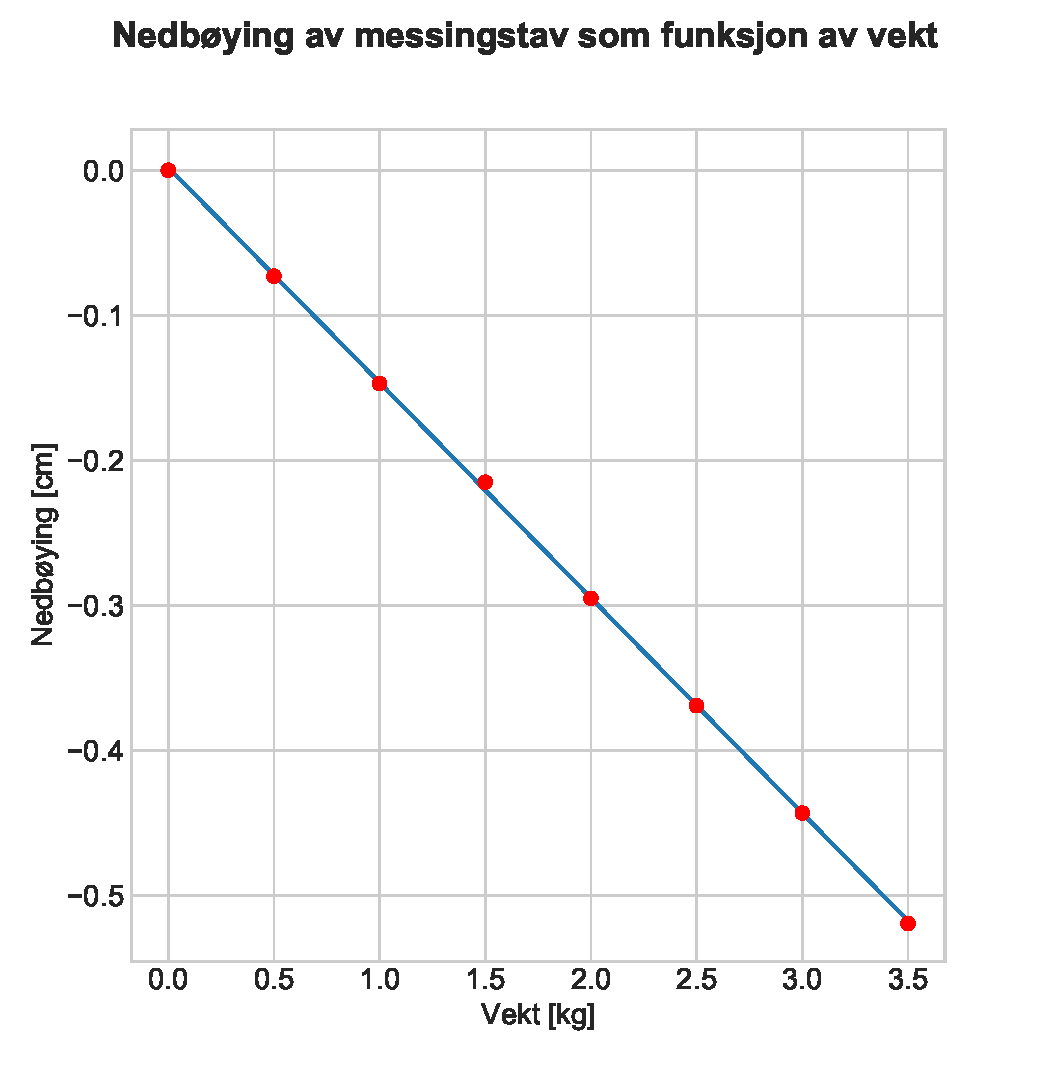
\includegraphics[scale=0.4]{nedbojing.pdf}
  \caption{Målinger gjort av nedbøyingen av staven $h$ som funksjon av lasten $m$ vi fester på midten av staven. De røde sirklene er målepunktene, og den blå linja er minstekvadraters lineærtilpassning.}
  \label{data}
\end{figure}
Siden det er vanskelig å se hvordan usikkerheten til målingene er iforhold til usikkerheten i stigningstallet i figuren ovenfor \vref{data} er differansen mellom målt utslag og lineærregresjonen plottet for alle målepunktene i figur \vref{data_usikker}.
\begin{figure}[h!]
  \centering
  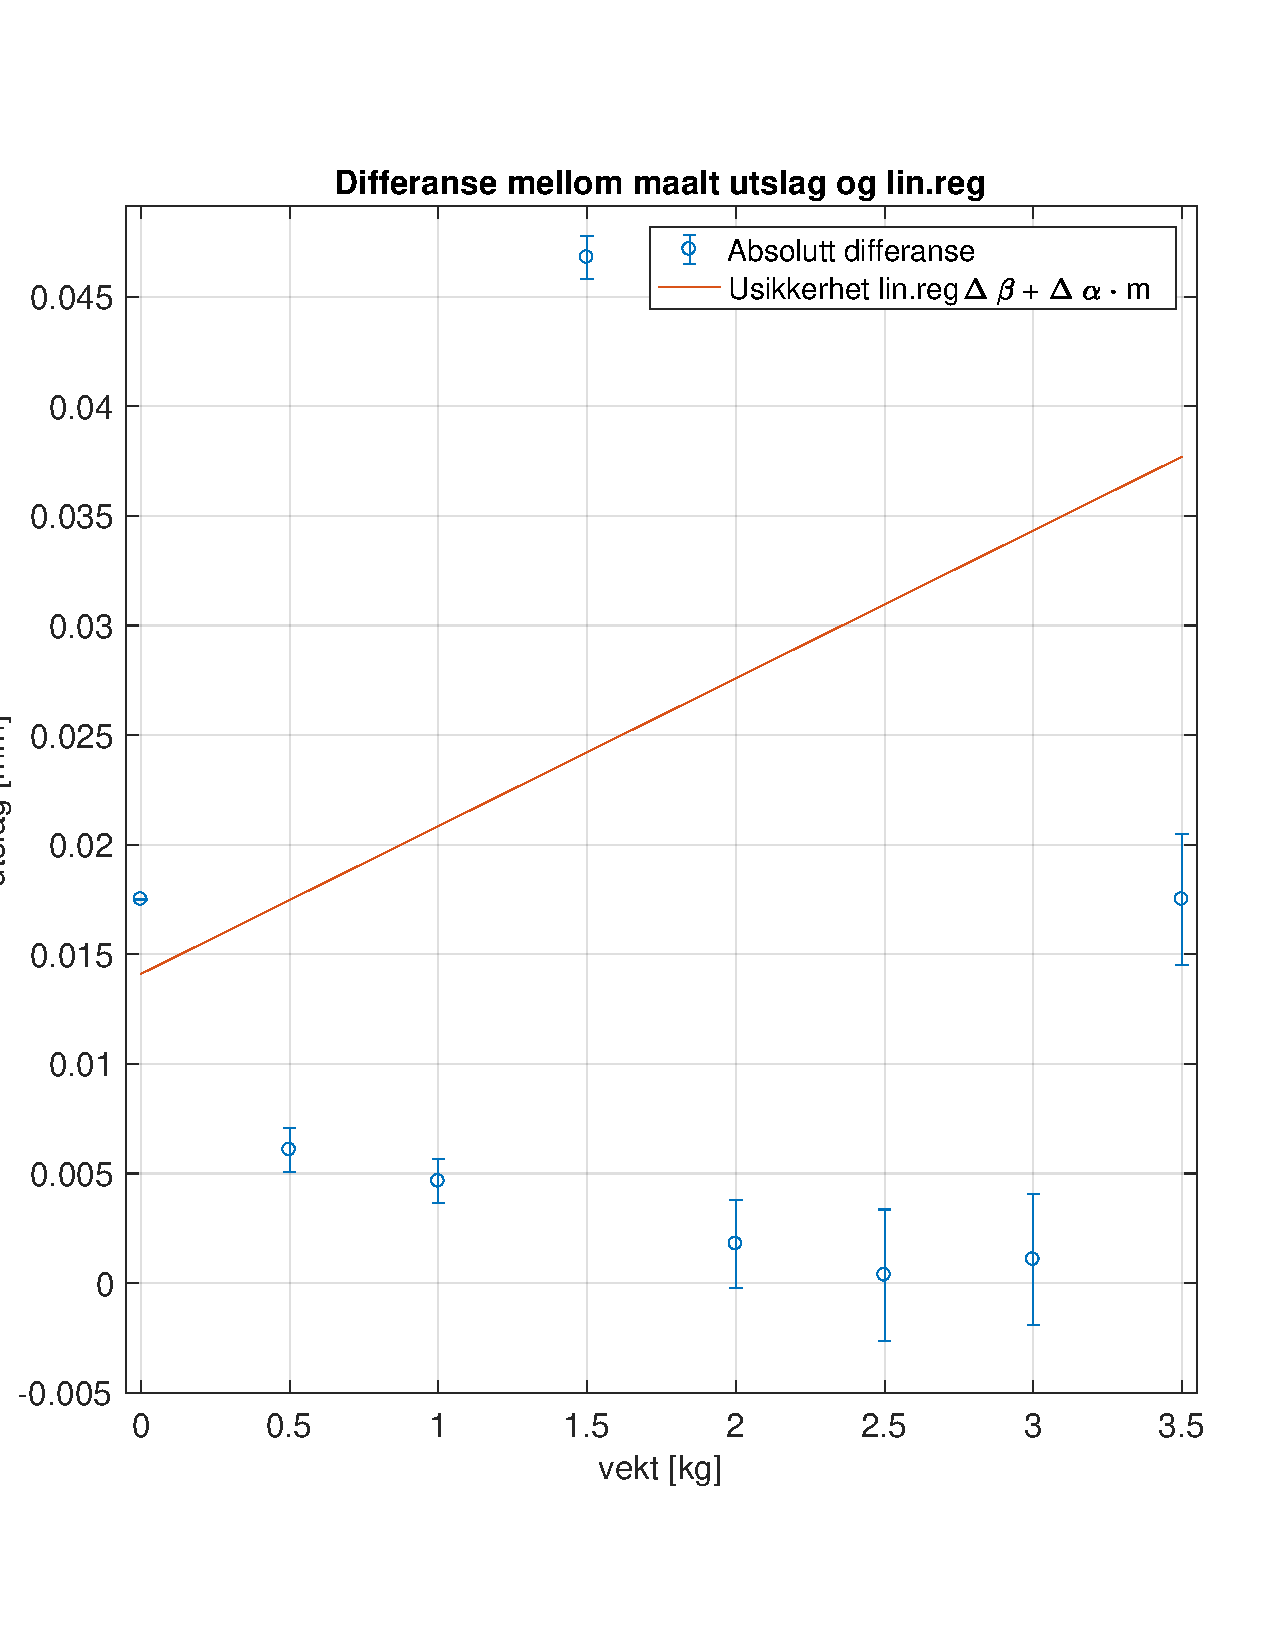
\includegraphics[scale=0.4]{usikkerhet.pdf}
  \caption{Absolutt differanse mellom målinger og lineærregresjonen til målingene.}
  \label{data_usikker}
\end{figure}
Ved å sette inn for diameteren og lengden fra tabell \vref{stav}, og tyngdeakselerasjonen og stigningstallet, inn i \eqref{young3} finner vi at $E=\SI{110\pm1}{\giga\pascal}$. Usikkerheten er beregnet fra likning \eqref{uncertenty1}, hvor vi har brukt usikkerheten i målingene nevnt ovenfor.
\subsection{Måling av utbredelseshastigheten til bølger}
Med denne metoden bruker vi likning \eqref{young5} for å beregne elastisitetsmodulen til messingstaven. For å beregne denne trenger vi igjen de geometriske størrelsene til staven vist i tabell \vref{stav}, men nå tregner vi ikke tyngdeakselerasjonen. Istedenfor tyngdeakselrasjonen trenger vi frekvensen som oppstår når vi slår på staven.
Vi gjorde flere målinger av frekvensen til bølgene som oppsto ved å slå på staven. Den fouriertransformerte av lyden mikrofonen tok opp på en av målingene er vist i figur \vref{fourier}. Fra å se på den fouriertransformerte ser vi at vi har en svært dominerende frekvens på $\SI{1207.1}{\hertz}$. Området rundt denne frekvens er tilnærmet lik null, og vi har litt støy for lave frekvenser under $\SI{100}{\hertz}$. Samplingstiden under eksperimentet var på $\SI{10}{\second}$ som gir oss en oppløsning på $\SI{0.1}{\hertz}$. Ved å ta med usikkerheten får vi derfor at frekvens til bølgen i staven er på $1207.1\pm\SI{0.1}{\hertz}$. Det ble gjort flere målinger av det samme, og på alle fikk vi samme frekvens.
\begin{figure}[h!]
  \centering
  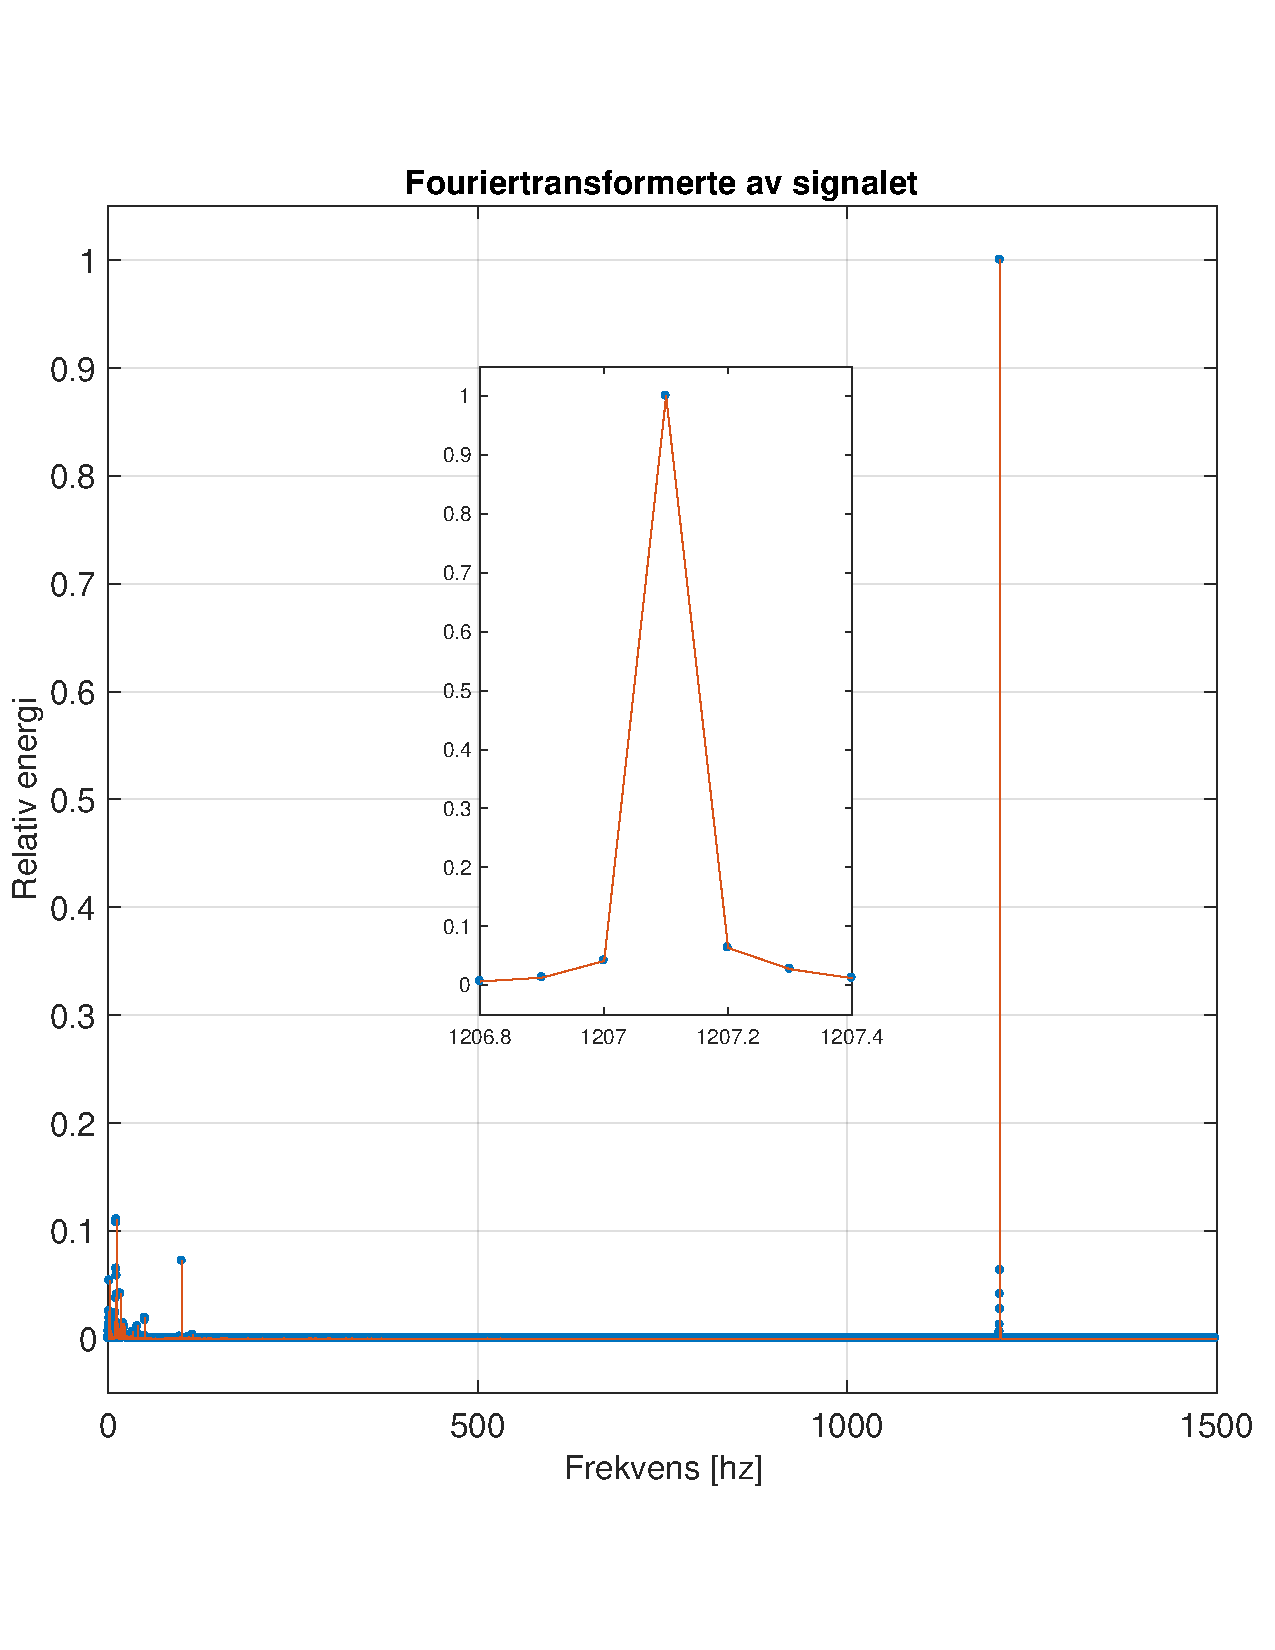
\includegraphics[scale=0.4]{fourier.pdf}
  \caption{Den fouriertransformerte av lyden motatt fra mikrofonen for en av målingene. I figuren er det inkludert et zoomet inn område rundt der frekvens ligger for å vise fram oppløsningen på målingene.}
  \label{fourier}
\end{figure}
Vi målte også frekvensen til bølgen ved å lete etter svevninger i lyden. Vi brukte derfor \eqref{young6} med elastisitetsmodulen vi fant ved å måle nedbøyingen til staven til å finne at grunnfrekvensen burde ligge på rundt $\SI{1211}{\hertz}$. Ved å bruke dette som startspunkt for å lete etter når perioden på svevningen økte eller minkte klarte vi å bestemme at frekvensen var på $\SI{1207.0}{\hertz}$. Under bruk av denne metoden brukte vi hørselen vår, og vi klarte å skille svevningen for frekvenser med en differanse på $\SI{0.2}{\hertz}$, vi får derfor en usikkerhet lik denne verdien. Ved svevning fant vi altså at frekvensen var på $1207\pm\SI{0.2}{\hertz}$.\\
For å beregne elastisitetsmodulen kommer vi til å bruke verdien og usikkerheten vi fant for frekvensen ved å bruke mikorofon og fouriertransformasjon. Ved å sette inn denne verdien, samt verdien vi målte for masse, lengde og diameter, vist i tabell \vref{stav}, i \eqref{young5}, får vi at elastisitetsmodulen er $E = \SI{109.3\pm0.3}{\giga\pascal}$. Usikkerheten er beregnet fra \eqref{uncertenty2}, hvor vi har brukt usikkerheten i målingene nevnt ovenfor.
\subsection{Usikkerheter}
Vi kan nå teste om ulikheten \eqref{usikk1} er tilfredstilt ved å beregne differansen mellom de to verdiene vi har for elastistetsmodulen, og usikkerheten i differeansen som er gitt av \eqref{usikk2}. Ved å gjøre disse beregningene finner vi at $D = \SI{0.7}{\giga\pascal}$, og at $\Delta D = \SI{1.1}{\giga\pascal}$. Altså er $D<\Delta D$, som betyr at differansenen mellom elastisitetsmodulen vi fikk med de to forskjellige metodene kommer av tilfeldige feil og måleusikkerheter.
\section{Diskusjon}
Under kalibreringen av vekten med presisjonslodddene kunne vi merke et utslag i balansevekten under en masseendring av $0.1$ gram, men vi merket at balansevekten var svært sensitiv til hvor på vektene loddene var på plassert. Med asymetri målte vi en vektforskjell på $0.6$g, og det er derfor en større usikkerhet i målingene enn presisjonen til instrumentet. Det var lett å unngå assymetri når vi kalibrerte med ett presisjonslodd, men måtte vi bruke to presisjonslodd i kalibreringen var det vanskeligere å garantere symetri på vekten. På grunn av dette ble usikkerheten til vekten, for loddene som trengte flere presisjonslodd for å kalibreres, større enn presisjonen til vekten.\\

Målingene for nedbøyingen av staven som funksjon av belastningen er vist i figur \vref{data}. I denne figuren er det vanskelig å se hvordan målingene, og usikkerheten til målingene, står iforhold til stigningstallet og usikkerheten i stigningstallet. Dette er derfor vist tydeligere i figur \vref{data_usikker}. I denne figuren ser vi at alle målingene, utenom en, ligger innenfor usikkerheten. Dette gjelder uavhengig av om vi tar med usikkerheten i målingen eller ikke. Vi ser også at nedbøyingen til staven når lasten er på $\SI{1.5}{\kilo\gram}$ avviker, godt utenfor usikkerheter, fra lineærregresjonen. Det forventes at en $\sigma$ av målingene, det vil si rundt $68\%$, burde ligge innenfor usikkerheten i stigningstallet, og det gjør det, men det store avviket kan tyde på at det var noe systematisk feil som skjedde under målingen av nedbøyingen med akkurat denne lasten. Det hadde vært ønskelig å oppdage dette avviket under eksperimentet slik at vi kunne gjort flere målinger med denne lasten, og lett etter mulige feil som kan ha påvirket målingen.\\
Utenom denne målingen er eksperimentet gjennomført godt beskyttet fra systematiske feil. Målingene av størrelsene til staven ble gjennomført flere ganger, lydopptak fra slaget på staven ble gjort flere ganger og vi fikk et lineært forhold mellom bøying av stav og belastning. Eksperimentet var godt kontrolert, og vi analyserte resultatene våre underveis for å sjekke at målingene ga mening før vi fortsatte. De tilfeldig feilene har påvirket målingene og vi har tatt hensyn til dette med usikkerheten til de to verdiene vi fant for elastistetsmodulen. Siden usikkerheten i differansen til elastistetmodulen er større enn differansen er det de tilfeldige feilene og måleusikkerhetene som forårsaker differansen. Vi kan derfor si at vi har overenstemmelse innenfor måleusikkerhetene. Dette gir oss en bekreftelse på at det ikke var merkbare systematiske feil tilstede under eksperimentet.
\\De to metodene ga oss det samme svaret, men med litt over en faktor $3$ forskjell i usikkerheten mellom de to metodene. Årsaken til den store forskjellen i usikkerhet er at målingene gjort med meterstokk er mye mindre presise enn de andre målingene. På grunn av dette vil metoden som hviler mest på målinger gjort av en meterstokk ha de største usikkerhetene. For metoden som bruker målingen av nedbøyingen til staven er avstanden mellom knivene svært viktig for elastisitetsmodulen, og går derfor som avstanden i tredje potens. Metoden der man bruker utbredelseshastigheten til bølgen for å beregne elastisitetsmodulen kanseleres lengden i utregningen av uttrykket slik at lengden på staven går i første potens. Siden meterstokken er det desidert største bidraget til usikkerheten fører en faktor $3$ i bidraget fra denne usikkerheten til et stort utslag i den endelige usikkerheten. Det er dette som har forårsaket den store forskjellen i usikkerhetene til resultatet. Det burde derfor brukes en mer presis måte å beregne lengden til staven og avstanden mellom knivene neste gang eksperimentet blir gjennomført for å redusere denne usikkerheten.
\section{Konklusjon}
En god fysisk modell burde kunne beskrive flere fenomener med så få parametere som mulig. I dette eksperimentet har vi vist at modellen for elastisitet klarer netopp dette ved å beskrive nedbøyingen til en stav som funksjon av belastningen på midtpunktet, og utbredelseshastigheten til bølger i samme stav med samme parameter, elastisitetsmodulen.
Ved å måle nedbøyingen som funksjon av last, og de geometriske størrelsene til staven, fant vi at elastisitetsmodulen er $E=\SI{110\pm1}{\giga\pascal}$.
Ved å fokusere på en bestemt bølgelengde klarer vi å bestemme utbredelseshastigheten ved å måle frekvensen til lydbølgen med en mikrofon. Verdien til frekvensen sammen med massen, lengde og diameter gir oss muligheten til å beregne at elastisitetsmodulen er $\SI{109.3\pm0.3}{\giga\pascal}$.
De to verdiene vi har funnet for elastisitetsmodulen har en differanse på $D = \SI{0.7\pm1.1}{\giga\pascal}$. Som vi ser er usikkerheten i differansen større en differansen, dette betyr at elastisitetsmodulene er like, men avviker på grunn av måleusikkerheter. Ved å ta utgangspunkt i to forskjellige fenomener har vi beregnet to forskjellige verdiene for elastisitetsmodulen som har overenstemmelse innenfor måleusikkerhetene.
\subsubsection*{Utstyrsliste}
\begin{itemize}
\label{utstyr}
\item meterstokk - Hultafors
\item skyvelær - Cocraft Micrometer
\item balansevekt - Ohaus Triple Beam Balance dial-o-gram
\item Måleur - Baker
\item opphengningsstativ
\item aluminiumstav
\item mikrofon
\end{itemize}
\begin{thebibliography}{9}
\bibitem{squires}
Squires, G.L. \emph{Practical Physics}, Cambridge University Press, 2001.
\bibitem{oppgave}
Fysisk institutt \emph{Elastisitet}, Universitetet i Oslo, februar 2018.
\bibitem{gravity}
W. J. Hinze, R. R. B. von Frese; A. H. Saad \emph{Gravity and Magnetic Exploration: Principles, Practices, and Applications}, Cambridge university press, 2013.
\bibitem{gronn}
Øyvind Grøn \emph{elastisitet – fysikk} \url{https://snl.no/elastisitet_-_fysikk} hentet 03.04.2018.
\end{thebibliography}
\end{document}
